\documentclass[12pt,a4paper]{article}

% Vietnamese support for pdflatex (Overleaf default)
\usepackage[utf8]{inputenc}
\usepackage[T5]{fontenc}
\usepackage[vietnamese]{babel}

\usepackage{graphicx}
\usepackage{booktabs}
\usepackage{geometry}
\usepackage{enumitem}
\usepackage{xcolor}
\usepackage{titlesec}
\usepackage{hyperref}
\usepackage{array}
\usepackage{float}

\geometry{top=2cm, bottom=2cm, left=2.5cm, right=2.5cm}

\definecolor{darkgreen}{RGB}{5, 150, 105}
\titleformat{\section}{\Large\bfseries\color{darkgreen}}{\thesection}{1em}{}
\titleformat{\subsection}{\large\bfseries}{\thesubsection}{1em}{}
\pagestyle{plain}

\begin{document}

\begin{center}
    {\LARGE\bfseries\color{darkgreen} GreenVision AI}\\[0.3cm]
    {\Large Hệ thống tối ưu hóa năng lượng thông minh bằng Trí tuệ nhân tạo và IoT}\\[1.5cm]
    \rule{\textwidth}{0.5pt}\\[0.3cm]
    {\large\bfseries BẢN MÔ TẢ Ý TƯỞNG SÁNG KIẾN}\\[0.3cm]
    \rule{\textwidth}{0.5pt}\\[2cm]
\end{center}

\section{Mô tả ý tưởng sáng kiến}

\subsection{Nhóm đối tượng hướng tới}

Hệ thống GreenVision AI hướng tới các nhóm đối tượng sau:

\begin{itemize}[leftmargin=1.5cm]
    \item \textbf{Quản lý nhà trường, trường đại học:} Giám sát tiêu thụ năng lượng tại phòng học, thư viện, phòng máy tính, ký túc xá.
    \item \textbf{Ban quản lý tòa nhà, văn phòng:} Tối ưu hóa chi phí điện tại các cơ sở phòng làm việc.
    \item \textbf{Đơn vị vận hành cơ sở hạ tầng:} Phát hiện sớm tình trạng lãng phí năng lượng để can thiệp kịp thời.
\end{itemize}

\subsection{Vấn đề cụ thể}

Tại các trường học và tòa nhà công cộng, điện năng bị lãng phí nghiêm trọng do ba nguyên nhân chính:

\begin{enumerate}[leftmargin=1.5cm]
    \item \textbf{Thiết bị hoạt động khi không cần thiết:} Đèn và điều hòa vẫn bật khi phòng trống.
    \item \textbf{Thiếu hệ thống giám sát tự động:} Không có công cụ theo dõi tiêu thụ năng lượng theo thời gian thực.
    \item \textbf{Phụ thuộc vào thao tác thủ công:} Việc tắt/mở thiết bị hoàn toàn dựa vào người dùng, dễ quên tắt khi rời phòng.
\end{enumerate}

\subsection{Giải pháp}

GreenVision AI là hệ thống giám sát năng lượng thông minh:

\vspace{0.3cm}
\begin{center}
\begin{tabular}{>{\bfseries}p{4cm} p{10cm}}
    \toprule
    Thành phần & Mô tả \\
    \midrule
    Camera + YOLO & Phát hiện và đếm số người trong phòng theo thời gian thực \\
    Cảm biến IoT & Thu thập dữ liệu môi trường: chuyển động, nhiệt độ, ánh sáng, công suất điện \\
    Cơ sở dữ liệu & Lưu trữ lịch sử để phân tích và biểu đồ \\
    Dashboard Web & Hiển thị chỉ tiêu năng lượng, số người, cảnh báo \\
    Phát hiện bất thường & Cảnh báo khi phòng trống nhưng đèn vẫn bật \\
    \bottomrule
\end{tabular}
\end{center}

\vspace{0.5cm}
\textbf{Quy trình hoạt động:}

\begin{enumerate}[leftmargin=1.5cm]
    \item Camera quan sát phòng $\rightarrow$ mô hình AI phát hiện người $\rightarrow$ đếm số người
    \item Cảm biến IoT đo nhiệt độ, ánh sáng, công suất, chuyển động
    \item Dữ liệu được gửi về máy chủ, lưu vào cơ sở dữ liệu
    \item Dashboard hiển thị dữ liệu theo thời gian thực qua WebSocket
    \item Nếu phòng trống + đèn bật + công suất cao $\rightarrow$ cảnh báo lãng phí
\end{enumerate}

\subsection{Cách yếu tố AI được lồng ghép}

\noindent
\begin{minipage}[t]{0.48\textwidth}
\textbf{Lớp 1 -- Nhận diện người (Computer Vision):}
\begin{itemize}[leftmargin=1.2cm]
    \item Mô hình YOLOv8 (Ultralytics) -- kiến trúc deep learning phát hiện đối tượng
    \item Huấn luyện trên bộ dữ liệu 3 nguồn: Kaggle, HuggingFace, Roboflow
    \item Tổng $\sim$3.300 ảnh gốc, augment lên $\sim$10.000 ảnh
    \item Kết quả: mAP@0.5 $>$ 0.9, chạy trên CPU
\end{itemize}
\end{minipage}
\hfill
\begin{minipage}[t]{0.48\textwidth}
\textbf{Lớp 2 -- Phát hiện bất thường năng lượng:}
\begin{itemize}[leftmargin=1.2cm]
    \item Phân tích dữ liệu cảm biến kết hợp nhận diện người
    \item Phòng trống + đèn bật + công suất cao $\rightarrow$ cảnh báo
    \item Tích hợp camera + sensor để xác minh
    \item Hiển thị cảnh báo realtime trên dashboard
\end{itemize}
\end{minipage}

\vspace{0.4cm}
\begin{figure}[H]
\centering
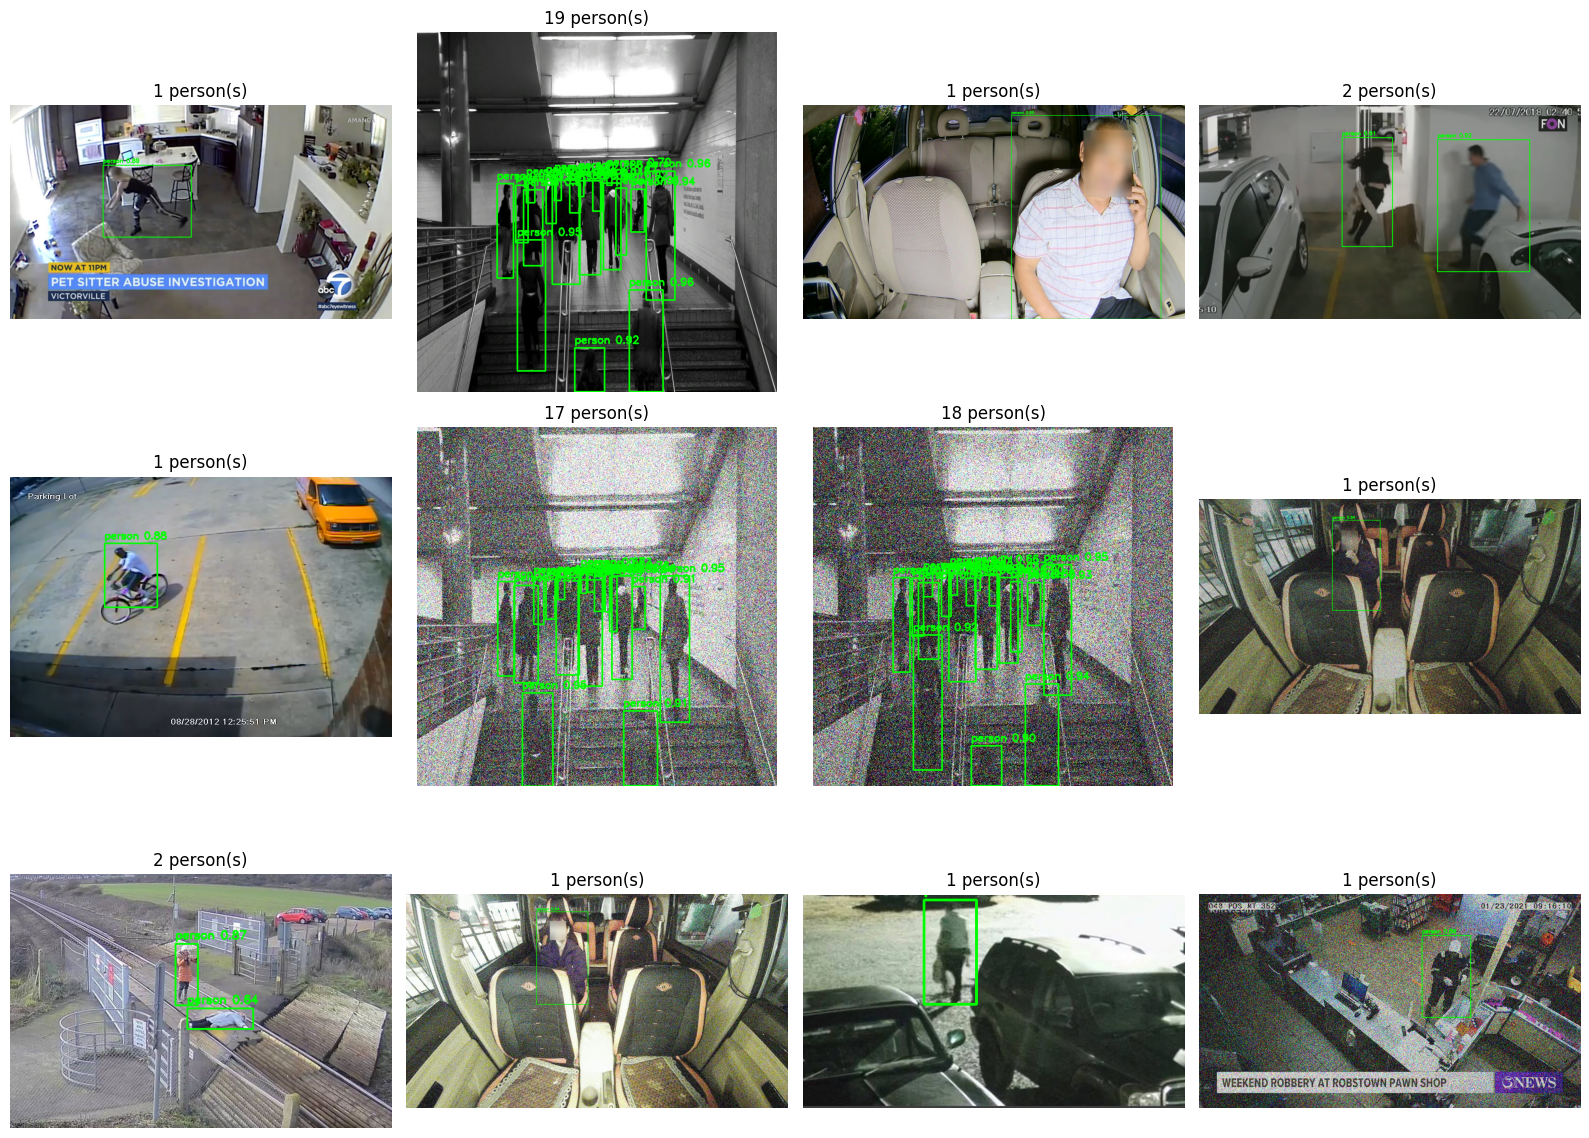
\includegraphics[width=0.7\textwidth]{detection.png}
\caption{AI phát hiện người -- YOLOv8 bounding box trên video stream}
\end{figure}

\section{Sản phẩm minh họa}

\subsection{Mô hình}

Hệ thống được triển khai dưới dạng web application, có thể truy cập trực tiếp tại:

\begin{center}
\url{https://duongphamminhdung.github.io/GreenVision/}
\end{center}

\textbf{Các chức năng chính:}

\begin{itemize}[leftmargin=1.5cm]
    \item Backend FastAPI + frontend React
    \item 5 phòng demo, dữ liệu sensor cập nhật mỗi 3 giây
    \item AI phát hiện người qua camera (YOLOv8)
    \item Cảnh báo lãng phí năng lượng khi phòng trống + công suất cao
\end{itemize}

\vspace{0.3cm}
\begin{figure}[H]
\centering
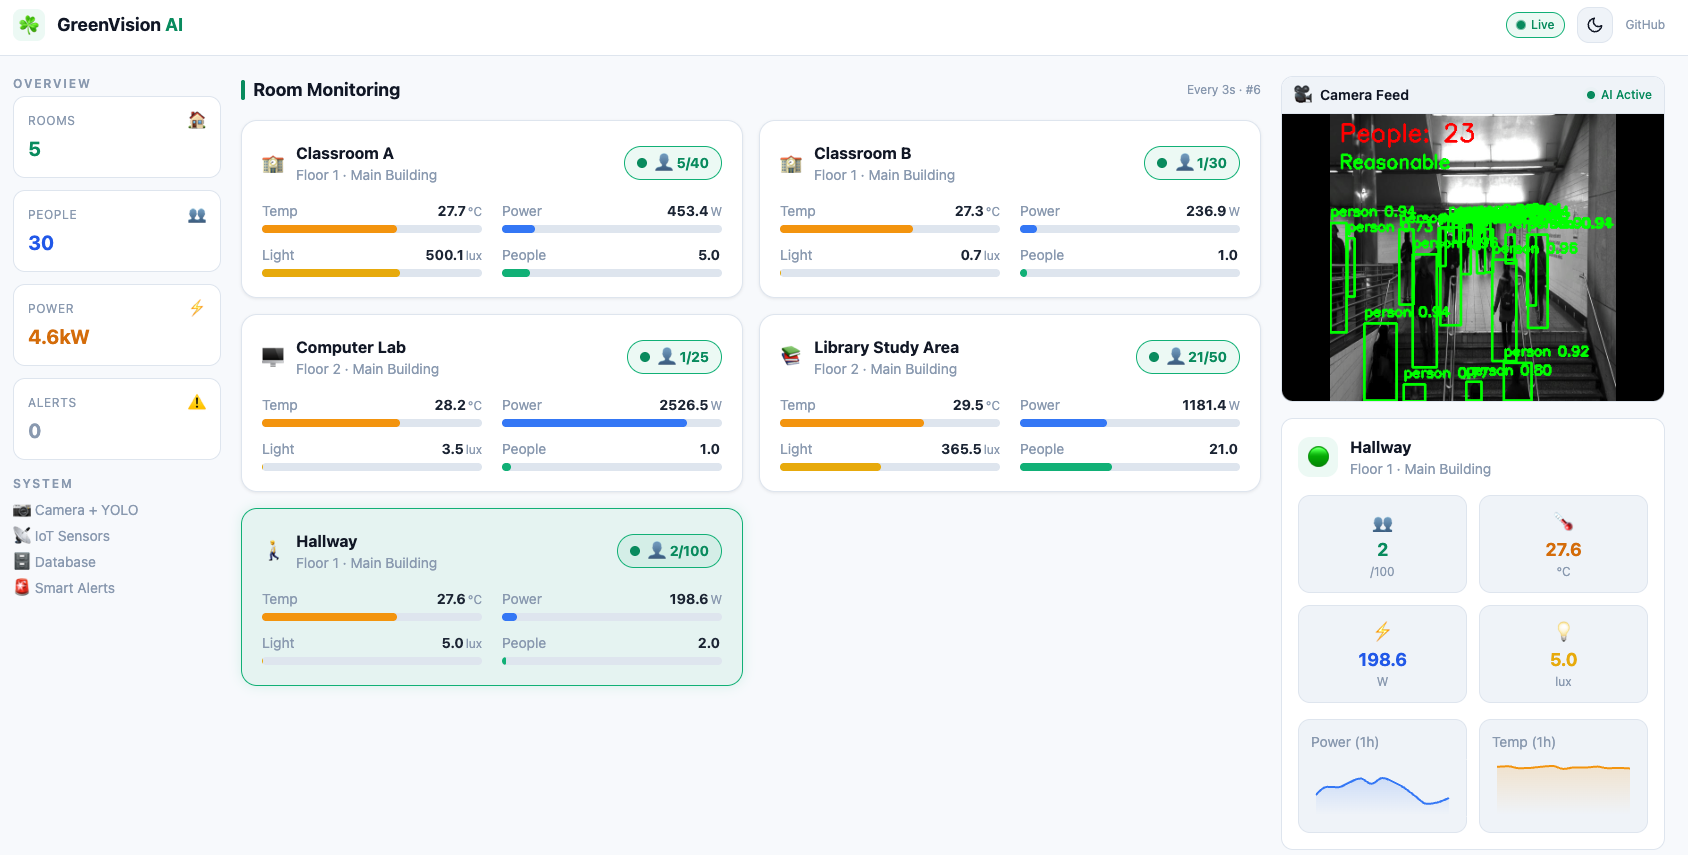
\includegraphics[width=0.9\textwidth]{dashboard.png}
\caption{Dashboard giám sát năng lượng -- hiển thị 6 phòng với dữ liệu sensor realtime, chế độ sáng/tối}
\end{figure}

\section{Thông tin đội thi}

\begin{center}
\begin{tabular}{lll}
    \toprule
    \multicolumn{3}{l}{\textbf{Đội GreenVision AI}} \\
    \midrule
    \textbf{Họ và tên} & \textbf{Trường} & \textbf{Vai trò} \\
    \midrule
    Dương Phạm Minh Dũng & VinUniversity & Backend \& AI \\
    Lê Nguyễn Vũ & National Economics University & Frontend \& UI/UX \\
    Đỗ Bảo Nam & Newton Highschool & IoT \& Data Analyst \\
    Lê Minh Quý & Newton Highschool & Hardware \& Testing \\
    Đặng Thành & Newton Highschool & Presentation \& Docs \\
    \bottomrule
\end{tabular}
\end{center}

\end{document}
